% Enable warnings about problematic code
\RequirePackage[l2tabu, orthodox]{nag}

\documentclass{resources/WeSTassignment}
\usepackage{tabularx}
\usepackage{booktabs}
\usepackage[utf8]{inputenc}
\usepackage{amsmath}
\usepackage{graphics}
\usepackage{graphicx}
\usepackage{changebar}
\usepackage{latexsym}
\usepackage{stmaryrd}
\usepackage{booktabs}
\usepackage{amsmath}
\usepackage{wasysym}
\usepackage[export]{adjustbox}
\usepackage[thinlines]{easytable}
\usepackage{framed}
\usepackage{color}
\usepackage{footnote}
\usepackage{listings}
\usepackage{framed}
\usepackage{tikz}
%\usepackage[table]{xcolor}

% The lecture title, e.g. "Web Information Retrieval".
\lecture{Machine Learning and Data Mining}
% The names of the lecturer and the instructor(s)
\author{%
  Raphael Menges\\{\normalsize\mailto{raphaelmenges@uni-koblenz.de}} 
}
% Assignment number.
\assignmentnumber{1}
% Institute of lecture.
\institute{%
  Institute of Web Science and Technologies\\%
  Department of Computer Science\\%
  University of Koblenz-Landau%
}
% Date until students should submit their solutions.
\datesubmission{16.11.2020, CEST 23:59}
% Date on which the assignments will be discussed in the tutorial.

% Specify bib file location.
\addbibresource{bibliography.bib}

\begin{document}

\maketitle
The exercises in this assignment are of theoretical nature and may not be solved by
execution of high-level Python commands but through manual step-by-step calculations which must be included in submissions. For this assignment it is also allowed
to upload a single .pdf file generated from LATEX code or scanned and compressed (!)
handwritten solutions. \\
\section{Statistics\hfill{18 points}}
\subsection{\hfill{6 points}}
 

\subsection{\hfill{6 points}}


\section{Error Calculation \hfill{12 points}}
You are given many computed outputs y\textsubscript{i} and desired outcomes \^y\textsubscript{i}.Provide the following error measures in regards to y\textsubscript{i} and \^y\textsubscript{i} by writing down their formula and a short description about their characteristics, i.e., the behavior in regard to the difference between computed and desired outcome.
\subsection{Sum of Square Error (SSE)}
\[ SSE = \sum_{i=1}^{n} (y_i-\hat{y_i} )^2 \]
y\textsubscript{i} : computed output \\
\^y\textsubscript{i} : desired output
\begin{figure}[htbp]
\centerline{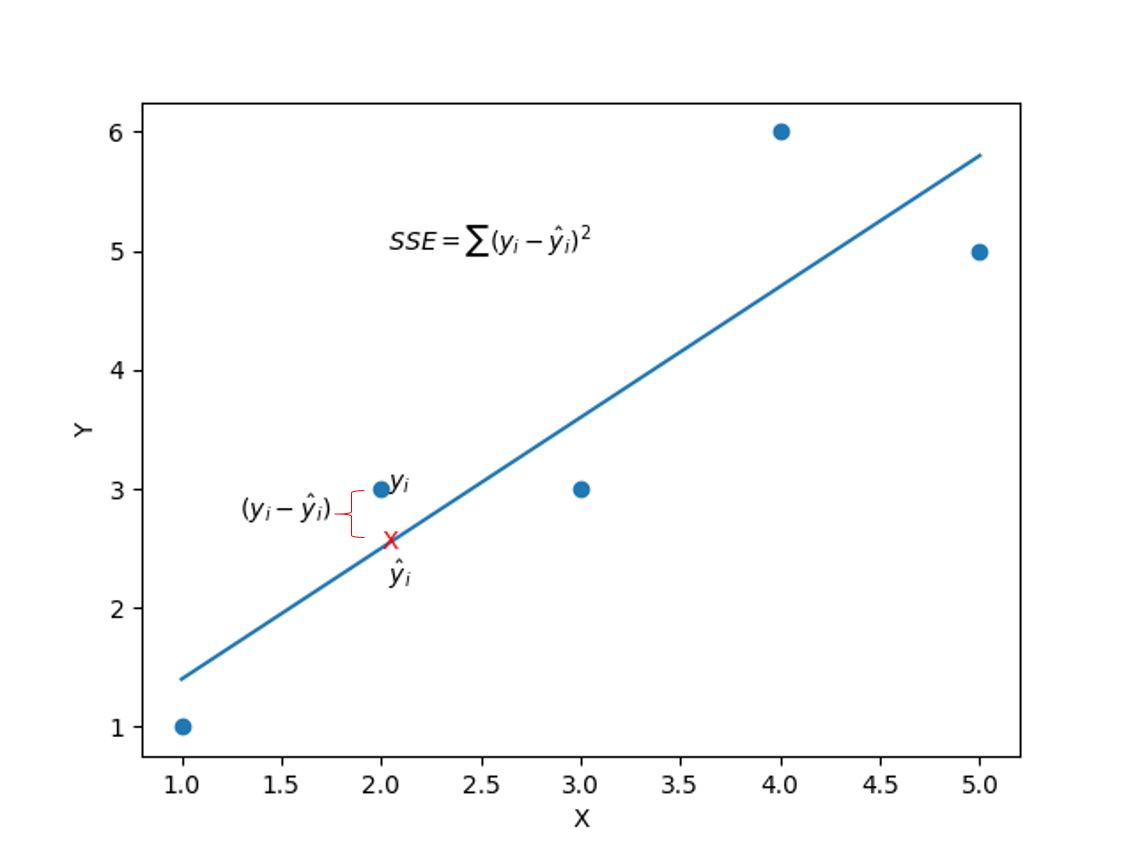
\includegraphics[scale=.5]{./resources/sse.png}}
\caption{sum of square error.}
\label{fig}
\end{figure}
\begin{itemize}
\item The error will be the summation of differences squared between y\textsubscript{i} (computed value) and \^y\textsubscript{i} (actual value).We compute how far away is our predicted value from actual value.
\item Positive terms cancelling out negative terms is avoided by squaring the difference.
\item We can differentiate SSE loss  function at all points which serves a greater advantage for mathematical optimisations( we obtain optimum point by differentiating the function and equating it to zero)
\end{itemize}
\subsection{Mean Square Error(MSE)}
\[ MSE = \sum_{i=1}^{n}\frac{1}{n} (y_i-\hat{y_i} )^2 \]
\begin{itemize}
	\item MSE is the quadratic loss function, which squares and subsequently
averages the various errors
	\item In MSE, squaring the error gives more weight to larger errors than smaller ones and thereby penalising them.
  
\end{itemize}
\subsection{ Root Mean Square Error (MSE)}
\[ RMSE =\sqrt{ \sum_{i=1}^{n}\frac{1}{n} (y_i-\hat{y_i} )^2} \]
\begin{itemize}
\item RMSE is the standard deviation of residuals from the best fit line (regression). It gives us an overview of how concentrated these residual points are around the line of best fit.
\item The triangle inequality is satisfied by RMSE, which is required for a distance function metric
\item RMSE penalises large errors.
\end{itemize}
\subsection{Mean Absolute Error (MAE)}  
\[ MAE = \sum_{i=1}^{n}\frac{1}{n} |y_i-\hat{y_i}| \]
\begin{itemize}
\item The models performance is not accurately reflected by MAE metric when dealing with large error values, thus it does not necessarily penalise large errors.
\item When the dataset is small and we have large number of outliers, a loss function which is  less sensitive to outliers like MAE could be chosen.
\end{itemize}
\section{Research tasks \hfill {20 points}}
.
\subsection{Collision}


\subsection{IPv6}


\section{Routing Table \hfill {20 points}}










\end{document}